%% ===== removed from ch6 on 2026-08-17 : fig:ctrl:dls-loop =====
%% A third rendering of the teacher loop, after Equation (6.1) and
%% Figure 6.1. images/ch6_dls_controller.pdf remains in images/.

\begin{center}
  \begin{minipage}{\textwidth}
    \centering
    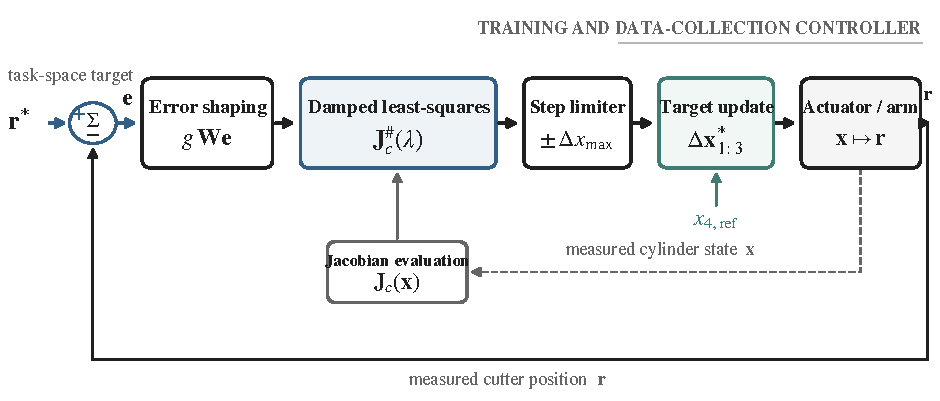
\includegraphics[width=\textwidth]{images/ch6_dls_controller}
    \captionof{figure}{Standard feedback realization of the DLS teacher in
    \eqref{eq:ctrl:teacher-dls}. The weighted task error is scaled, mapped to
    the first three cylinder coordinates by the measured damped inverse, and
    clipped. Cylinder~4 is held at its head-down reference. Cutter position
    closes the task-space loop and the measured cylinder state updates
    $\bm{J}_c$. The loop is used only for teaching and data collection, not at
    deployment.}
    \label{fig:ctrl:dls-loop}
  \end{minipage}
\end{center}
